We have prototyped static pair-wise lock set analysis in \textsc{Whoop}, a practical tool for automatic verification of data race freedom in Linux drivers written in C~\cite{kernighan1988c}. The tool's architecture is depicted in Figure~\ref{figure:toolchain}, and the whole toolchain can be summarised as follows:

\begin{figure}[tbp]
\centering
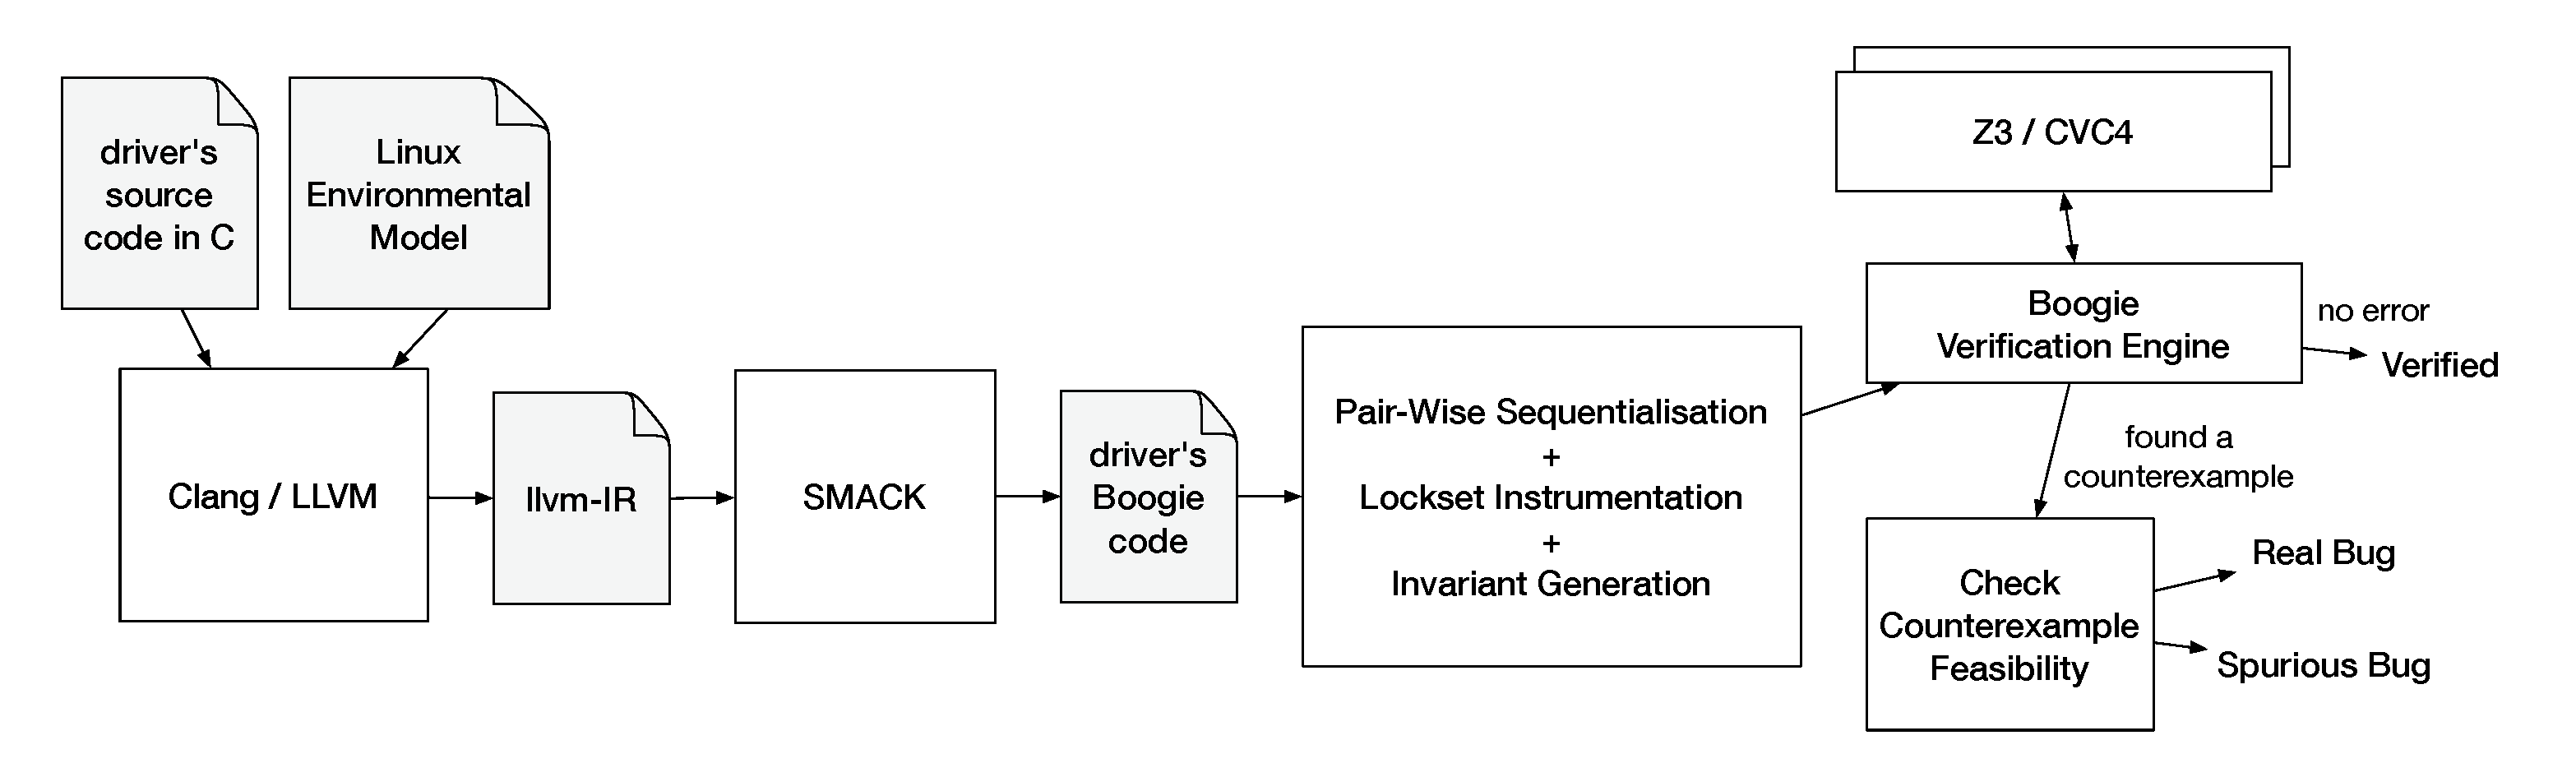
\includegraphics[width=.99\linewidth]{img/toolchain.pdf}
\caption{The \textsc{Whoop} architecture, which is powered by the Clang/LLVM and Boogie frameworks.}
\label{figure:toolchain}
\end{figure}

Initially, the device driver source code, together with a Linux environmental model\footnote{Stub header files required for compiling and subsequently analysing a device driver.}, is compiled to LLVM-IR using Clang/LLVM~\cite{lattner2004llvm}. Then, the LLVM-IR is compiled to the Boogie~\cite{barnett2006boogie} verification language using SMACK~\cite{rakamaric2008automatic}, an open source LLMV-IR to Boogie translator which can efficiently model heap manipulating programs. Next, the Boogie program is transformed into a sequentialised abstract program, using pair-wise sequentialisation and lock set instrumentation as discussed in Section~\ref{method}. Finally the abstract program is send to the Boogie verification engine, which generates verification conditions~\cite{barnett2005weakest} and discharges them to a theorem prover. Successful verification implies that the original driver is free of data races, while an error denotes a \emph{potential} data race.

\textsc{Whoop} is currently working on an unmodified network device driver (the RealTek r8169 which is part of the official Linux kernel distribution). Our immediate future work includes applying invariant generation to tame the effect of our coarse over-approximation. We also plan to introduce counterexample feasibility checking to evaluate if a reported bug is real or spurious. Towards this, we plan to feed a counterexample generated by \textsc{Whoop} into a precise bug finder, such as Corral~\cite{lal2012corral}, which will be guided only to execution paths that may manifest the bug, to either confirm it or discard it as a false positive.